\section{Case Study}\label{sec:case_study}

To illustrate the utility of \name we have implemented a number of
queries and transformations in the context of QL, a DSL for
questionnaires which has been implemented using Object Algebras
before~\cite{gouseti14extensible}.  QL is similar to MiniQL, except that
it additionally features an if-then-else construct, computed questions
(which will appear read only), and a richer expression language.  For
more information on the features of QL we refer
to~\cite{erdweg2013state}.

%% A questionnaire is rendered as an interactive form where, depending on user actions, new questions may appear, or values may be computed.
%% An example QL questionnaire is shown on the left of Figure~\ref{FIG:houseowning} together with its rendering on the right.

%% QL programs consist of lists of labeled, typed questions.
%% Questions can be answerable, meaning the user has to enter some data, or computed, in which case the question is defined by an expression.
%% A conditional if-then-else construct allows questions to visually appear only when a certain condition is true.

%% \begin{figure}[t]
%% \nocaptionrule
%% \hspace*{-5pt}\begin{minipage}{0.6\linewidth}
%% \begin{lstlisting}[language=ql]
%% form HouseOwning {
%%   soldHouse: "Did you sell a house?" boolean
%%   boughtHouse: "Did you buy a house?" boolean
%%   if (soldHouse) {
%%     sellingPrice: "Selling price:" integer
%%     privateDebt: "Private debts:" integer
%%     valueResidue: "Value residue:" integer
%%        = (sellingPrice - privateDebt)
%%   }
%% }
%% \end{lstlisting}
%% \end{minipage}
%% \begin{minipage}{0.5\linewidth}
%%   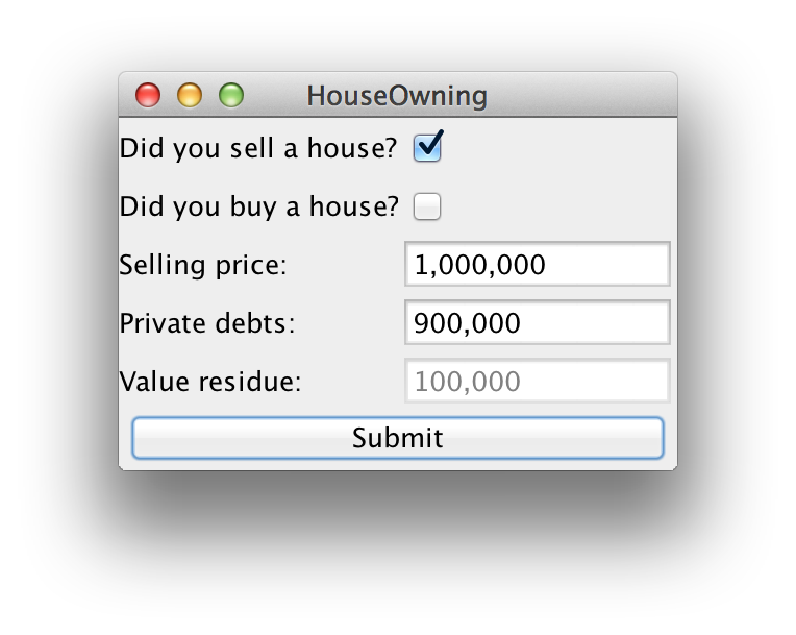
\includegraphics[width=\linewidth]{sections/screenshot}
%% \end{minipage}
%% \caption{Example QL questionnaire (left) and its rendering (right)}
%% \label{FIG:houseowning}
%% \end{figure}

\subsection{QL Queries and Transformations}

The queries extract derived information from a QL program, such as the set of used variables, the data and control dependencies between questions, and the global type environment.
The transformations include two transformations of language extensions to the base language.
The first realizes a simple desugaring of ``unless(c){...}'' to ``if(not(c)){...}''.
The second desugaring statically unfolds a constant bound loop construct (``repeat (i){...}'') and renames variables occurring below it accordingly.
Finally, we have implemented a simple rename variable operation, and a flattening normalizer which inlines the conditions of nested if-then constructs.

Table~\ref{TBL:qlresults} shows the number of cases that had to be overridden to implement each particular operation. The top row shows the number of  constructs for each syntactic category in QL (Exp, Stmt, and Form).
As can be seen, none of the operations required implementing all cases.
The last column shows the number of overridden cases as a percentage.
For this set of queries and transformations, almost no expression cases needed to be overridden, except the ``Var'' case in collect variables, rename variable and desugar ``repeat''\footnote{Note, however, that the dependency extraction queries reuse the collect variables query on expressions.}.
The cases required for desugaring include the case of the language extension (e.g. \lstinline{Unless} and \lstinline{Repeat}, respectively). These cases are not counted in the total in the first row but are used to compute the percentage.

\begin{table}[t]
  \centering\small
  \begin{tabular}{@{}llllr@{}}\toprule
    Operation            & Exp (18) & Stmt (5) & Form (1) & \%     \\\hline
    Collect variables    & 1        &          &          & 4\%  \\
    Data dependencies    &          & 3        & 1        & 17\% \\
    Control dependencies &          & 4        & 1        & 21\% \\
    Type environment     &          & 2        &          & 8\%  \\\hline
    Rename variable      & 1        & 2        &          & 13\% \\
    Inline conditions    &          & 4        &          & 17\% \\
    Desugar ``unless''   &          & 1        &          & 4\%  \\
    Desugar ``repeat''   & 1        & 3        &          & 16\% \\\bottomrule
  \end{tabular}
\nocaptionrule   \caption{Number of overriden cases per query and transformation in
    the context of the QL implementation\label{TBL:qlresults}.}
\end{table}

%% \def\rot#1{\rotatebox{90}{#1}}

%% \begin{table}[t]
%%   \centering
%%   \nocaptionrule
%%   \hspace*{-.05\textwidth}
%%   \begin{tabular}{lccccccccc}
%%     Sort & \rot{\#Cases} & \rot{Collect vars} & \rot{Data deps} & \rot{Control deps} & \rot{Type env} & \rot{Rename var} & \rot{Inline conds} & \rot{\texttt{unless}} & \rot{\texttt{repeat}} \\\hline
%%     Form & 1             &                    & 1               & 1                  &                &                  &                    &                       &                       \\
%%     Stmt & 5             &                    & 3               & 4                  & 2              & 2                & 4                  & 1                     & 3                     \\
%%     Exp  & 18            & 1                  &                 &                    &                & 1                &                    &                       & 1                     \\\hline
%%          &               & 4\%                & 17\%            & 21\%               & 8\%            & 13\%             & 17\%               & 4\%                   & 16\%                  \\
%%   \end{tabular}
%%   %\vspace*{.1in}
%%   \caption{Number of overridden cases per query and transformation in
%%     the context of the QL implementation\label{TBL:qlresults}}
%% \end{table}


%% \subsection{Extending queries and transformations}

%% Instead of desugaring language extensions to the base language it is also possible to treat them as first-class constructs and retroactively extend existing queries and transformations.
%% The framework permits to use  Java interface extension to achieve this in a fully type safe way.
%% Figure~\ref{inline_conds_unless} and Figure~\ref{controldeps_unless} show the extension of the inline conditions transformation and control dependencies query when extending QL with ``unless''.

%% \begin{figure}[tb]
%% \lstinputlisting[linerange=9-14]{../QL/src/_syb/trafo/InlineConditionsUnless.java} % APPLY:linerange=INLINECONDS_UNLESS
%% \vspace{-.1in}
%% \caption{Extending the inline-conditions transformation to deal with ``unless''}
%% \label{inline_conds_unless}
%% \end{figure}

%% \begin{figure}[tb]
%% \lstinputlisting[linerange=9-17]{../QL/src/_syb/query/ControlDepGraphUnless.java} % APPLY:linerange=CONTROLDEPS_UNLESS
%% \vspace{-.1in}
%% \caption{Extending the control-dependencies query to deal with ``unless''}
%% \label{controldeps_unless}
%% \end{figure}

%% Inlining of conditions across ``unless'' statements (Figure~\ref{inline_conds_unless}) is analogous to the implementation for ``if''.
%% It involves creating a conjunction of the input (\lstinline{guard}) and the negated condition and then passing it down the body of ``unless''. The result is the inlined version of the body.
%% The extension of the control dependencies (Figure~\ref{controldeps_unless}) query simply delegates to the implementation of ``if'' (\lstinline{iff}).

\subsection{Chaining Transformations}
\label{SECT:chaining}

A typical compiler consists of many transformations chained together in a pipeline.
\name transformations support this pattern by passing transformation algebras as the base algebra to the implementation of another transformation.
For instance, the desugar unless transformation desugars the ``unless'' statement to ``if'' statements in another algebra.
The latter can represent yet another transformation.

In the context of QL, ``unless'' desugaring, condition inlining and variable renaming can be chained together as follows:

  \lstinputlisting[linerange=170-172]{../QL/src/_syb/trafo/TestPipelining.java} % APPLY:linerange=PIPELINEQL

The chained transformation \lstinline{alg} first desugars ``unless'', then inlines conditions, and finally renames \lstinline{x}s to \lstinline{y}s.
The \lstinline{Rename} transformation gets as base algebra an instance of \lstinline{Format}, a pretty printer for QL.

The algebra \lstinline{alg} can now be used to create questionnaires:

  \lstinputlisting[linerange=176-179]{../QL/src/_syb/trafo/TestPipelining.java} % APPLY:linerange=PIPELINEQL_CALL

Since inlining is a contextual transformation, the result of constructing this simple questionnaire is a function object representing the ``to be inlined'' representation of the questionnaire after desugaring.
The {\small\texttt{IFor\-mat\-With\-Pre\-cedence}} and \lstinline{IFormat} types are  formatting operations, respectively representing expressions and statements; these types originate from the \lstinline{Format} algebra passed to \lstinline{Rename}.

Calling the function with a boolean expression representing \lstinline{true} will trigger inlining of conditions and renaming. The result is then a formatting object (\lstinline{IFormat}) which can be used to print out the transformed questionnaire:

  \begin{lstlisting}[language=ql]
  form myForm { if (true && !y) y "X?" boolean }
  \end{lstlisting}

\noindent As can be seen, the variable \lstinline{x} has been renamed to \lstinline{y}.
The (renamed) condition \lstinline{y} is now negated, because of the desugaring of ``unless''.
Finally, the result of inlining conditions can be observed from the conjunction in the \lstinline[language=ql]{if} statement.


\subsection{\name Performance vs Vanilla ASTs}

\begin{figure}[t]
  \nocaptionrule
  \hspace*{-.05\textwidth}
  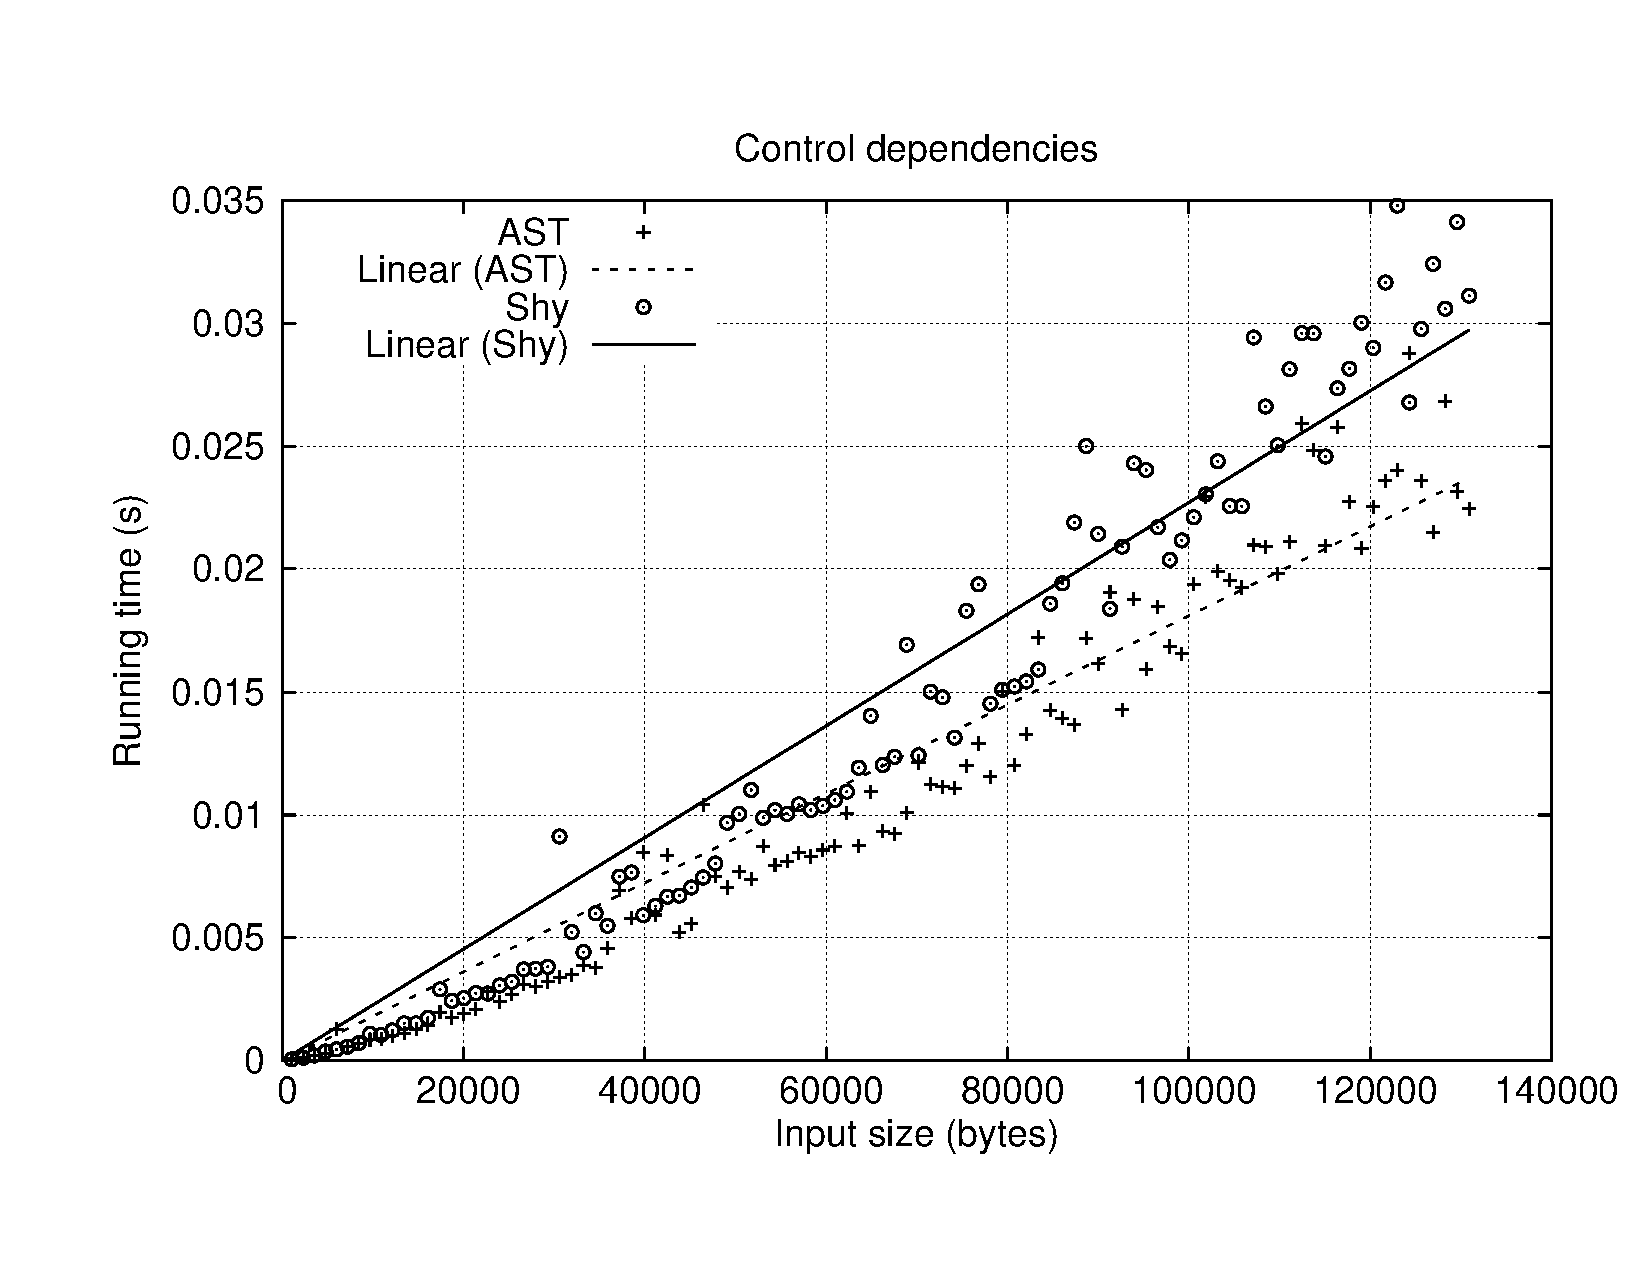
\includegraphics[width=0.56\textwidth]{plots/controldeps}
  \caption{Performance comparison of control dependencies query.\label{FIG:controlPerf}}
\end{figure}

We compared the performance characteristics of the operations implemented using \name with respect to vanilla implementations based on ordinary AST classes with ordinary methods representing the transformations and queries.
In the vanilla implementation, the program was parsed into an AST structure, and then the operation was invoked and measured.
In the case of the \name queries, constructing the ``AST'' corresponds to executing the query, so we measured that.
For context-dependent transformations, however, building the ``AST'' corresponds to constructing the function to execute the transformation, hence we only measured invoking this function.
The vanilla query implementations use the same monoid structures as in \name.

The operations were executed on progressively larger QL programs (up to 140Kb). The QL programs represent questionnaires describing a binary search problem (a number guessing game) and are automatically generated, with increasing search spaces. The benchmarks were executed on a 2.6GHz MacBook Pro Intel Core i5 with 8GB memory. The JVM was run in 64bit server mode and was given 4Gb of heapspace to minimize the effect of garbage collection pauses. Each benchmark was run without measuring first,  to warm-up the JVM. The measurements presented here do not include warm-up time.

The comparison of the control dependencies query is shown in Figure~\ref{FIG:controlPerf}.
The plot shows that the performance is quite comparable.
On average, the \name implementation of the query seems a little slower.
This is probably caused by the extensive use of interfaces in the \name framework, whereas the AST-based implementation only uses abstract and concrete classes.
%\tijs{NEED REFERENCE!!!!, but see: \url{http://stackoverflow.com/questions/6839943/why-are-interface-method-invocations-slower-than-concrete-invocations}}.
For transformations the performance difference is slightly more pronounced.
Figure~\ref{FIG:inlinePerf} shows the performance comparison of the inline conditions transformation.
The greater difference can be explained by the fact that creating a new structure in a \name transformation involves dynamically dispatched method calls instead of statically bound constructor calls.

\begin{figure}[t]
  \nocaptionrule
  \hspace*{-.05\textwidth}
  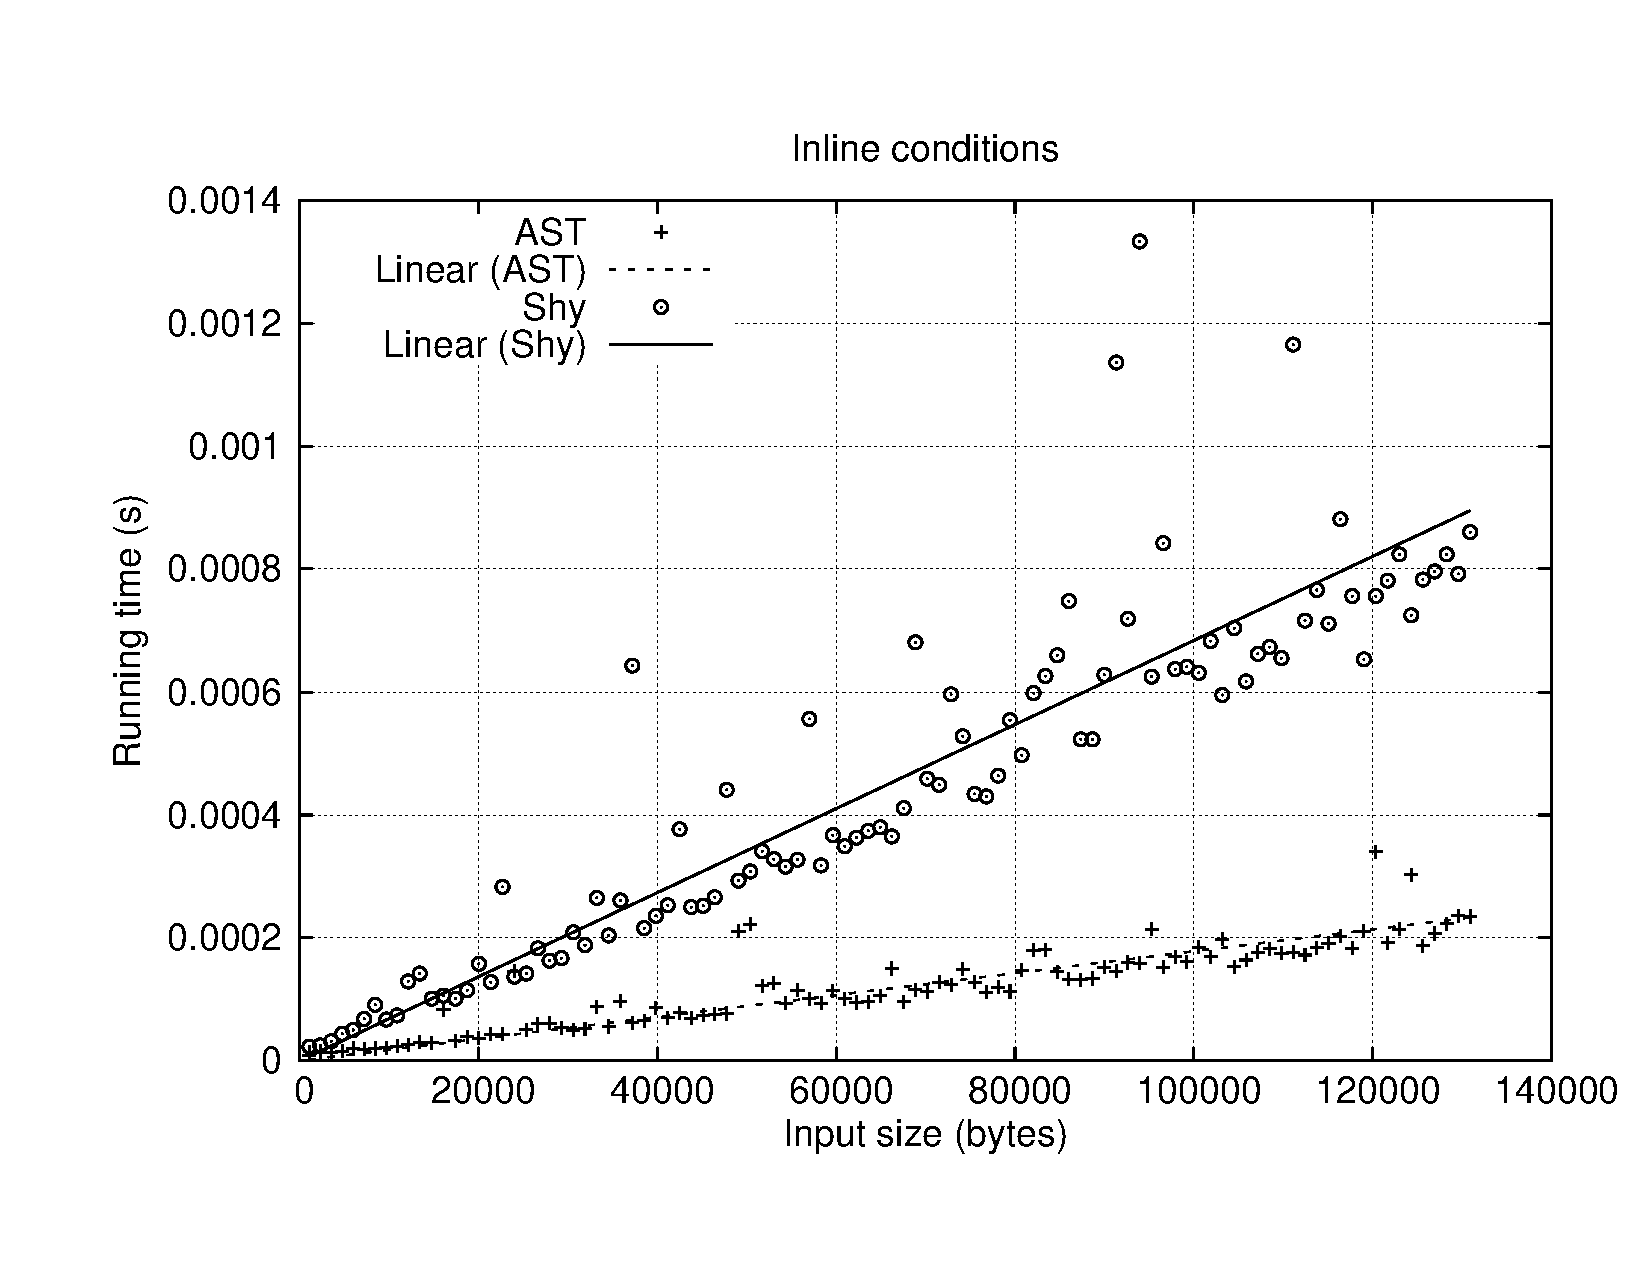
\includegraphics[width=0.56\textwidth]{plots/inline}
  \caption{Performance comparison of inline conditions transformation.\label{FIG:inlinePerf}}
\end{figure}





